%% abtex2-modelo-relatorio-tecnico.tex, v<VERSION> laurocesar
%% Copyright 2012-<COPYRIGHT_YEAR> by abnTeX2 group at http://www.abntex.net.br/ 
%%
%% This work may be distributed and/or modified under the
%% conditions of the LaTeX Project Public License, either version 1.3
%% of this license or (at your option) any later version.
%% The latest version of this license is in
%%   http://www.latex-project.org/lppl.txt
%% and version 1.3 or later is part of all distributions of LaTeX
%% version 2005/12/01 or later.
%%
%% This work has the LPPL maintenance status `maintained'.
%% 
%% The Current Maintainer of this work is the abnTeX2 team, led
%% by Lauro César Araujo. Further information are available on 
%% http://www.abntex.net.br/
%%
%% This work consists of the files abntex2-modelo-relatorio-tecnico.tex,
%% abntex2-modelo-include-comandos and abntex2-modelo-references.bib
%%

% ------------------------------------------------------------------------
% ------------------------------------------------------------------------
% abnTeX2: Modelo de Relatório Técnico/Acadêmico em conformidade com 
% ABNT NBR 10719:2015 Informação e documentação - Relatório técnico e/ou
% científico - Apresentação
% ------------------------------------------------------------------------ 
% ------------------------------------------------------------------------

\documentclass[
	% -- opções da classe memoir --
	12pt,				% tamanho da fonte
	openright,			% capítulos começam em pág ímpar (insere página vazia caso preciso)
	twoside,			% para impressão em recto e verso. Oposto a oneside
	a4paper,			% tamanho do papel. 
	% -- opções da classe abntex2 --
	%chapter=TITLE,		% títulos de capítulos convertidos em letras maiúsculas
	%section=TITLE,		% títulos de seções convertidos em letras maiúsculas
	%subsection=TITLE,	% títulos de subseções convertidos em letras maiúsculas
	%subsubsection=TITLE,% títulos de subsubseções convertidos em letras maiúsculas
	% -- opções do pacote babel --
	english,			% idioma adicional para hifenização
	french,				% idioma adicional para hifenização
	spanish,			% idioma adicional para hifenização
	brazil,				% o último idioma é o principal do documento
]{abntex2}


% ---
% PACOTES
% ---

% ---
% Pacotes fundamentais 
% ---
\usepackage{lmodern}			% Usa a fonte Latin Modern
\usepackage[T1]{fontenc}		% Selecao de codigos de fonte.
\usepackage[utf8]{inputenc}		% Codificacao do documento (conversão automática dos acentos)
\usepackage{indentfirst}		% Indenta o primeiro parágrafo de cada seção.
\usepackage{color}				% Controle das cores
\usepackage{graphicx}			% Inclusão de gráficos
\usepackage{microtype} 			% para melhorias de justificação
% ---

% ---
% Pacotes adicionais, usados no anexo do modelo de folha de identificação
% ---
\usepackage{multicol}
\usepackage{multirow}
% ---
	
% ---
% Pacotes adicionais, usados apenas no âmbito do Modelo Canônico do abnteX2
% ---
\usepackage{lipsum}				% para geração de dummy text
% ---

% ---
% Pacotes de citações
% ---
\usepackage[brazilian,hyperpageref]{backref}	 % Paginas com as citações na bibl
\usepackage[alf]{abntex2cite}	% Citações padrão ABNT

% --- 
% CONFIGURAÇÕES DE PACOTES
% --- 

% ---
% Configurações do pacote backref
% Usado sem a opção hyperpageref de backref
\renewcommand{\backrefpagesname}{Citado na(s) página(s):~}
% Texto padrão antes do número das páginas
\renewcommand{\backref}{}
% Define os textos da citação
\renewcommand*{\backrefalt}[4]{
	\ifcase #1 %
		Nenhuma citação no texto.%
	\or
		Citado na página #2.%
	\else
		Citado #1 vezes nas páginas #2.%
	\fi}%
% ---

% ---
% Informações de dados para CAPA e FOLHA DE ROSTO
% ---
\titulo{Optimização Bayesiana}
\autor{Douglas Braga \textbackslash{}~Felipe Sales}
\local{Brasil}
\data{31 dezembro, 2019}
\instituicao{}
\tipotrabalho{Relatório técnico}
% O preambulo deve conter o tipo do trabalho, o objetivo, 
% o nome da instituição e a área de concentração 
\preambulo{Modelo canônico de Relatório Técnico e/ou Científico em conformidade com
as normas ABNT apresentado à comunidade de usuários \LaTeX.}
% ---

% ---
% Configurações de aparência do PDF final


% alterando o aspecto da cor azul
\definecolor{blue}{RGB}{41,5,195}

% informações do PDF
\makeatletter
\hypersetup{
     	%pagebackref=true,
		  pdftitle={Optimização Bayesiana}, 
		  pdfauthor={Douglas Braga \textbackslash{} Felipe Sales},
    	pdfsubject={\imprimirpreambulo},
	    pdfcreator={LaTeX with abnTeX2},
		  pdfkeywords={abnt}{latex}{abntex}{abntex2}{relatório técnico}, 
		  colorlinks=true,       		% false: boxed links; true: colored links
    	linkcolor=blue,          	% color of internal links
    	citecolor=blue,        		% color of links to bibliography
    	filecolor=magenta,      		% color of file links
		  urlcolor=blue,
		  bookmarksdepth=4
}
\makeatother
% --- 

% --- 
% Espaçamentos entre linhas e parágrafos 
% --- 

% O tamanho do parágrafo é dado por:
\setlength{\parindent}{1.3cm}

% Controle do espaçamento entre um parágrafo e outro:
\setlength{\parskip}{0.2cm}  % tente também \onelineskip

% ---
% compila o indice
% ---
\makeindex
% ---

% ----
% Início do documento
% ----
\begin{document}


% Seleciona o idioma do documento (conforme pacotes do babel)
\selectlanguage{brazil}

% Retira espaço extra obsoleto entre as frases.
\frenchspacing 

% ----------------------------------------------------------
% ELEMENTOS PRÉ-TEXTUAIS
% ----------------------------------------------------------
% \pretextual

% ---
% Capa
% ---
\imprimircapa
% ---

% ---
% Folha de rosto
% (o * indica que haverá a ficha bibliográfica)
% ---
\imprimirfolhaderosto*

% ---
% Agradecimentos
% ---
\begin{agradecimentos}
  O agradecimento principal é direcionado a Youssef Cherem, autor do
  \nameref{formulado-identificacao}
  (\autopageref{formulado-identificacao}).
  
  Os agradecimentos especiais são direcionados ao Centro de Pesquisa em
  Arquitetura da Informação\footnote{\url{http://www.cpai.unb.br/}} da
  Universidade de Brasília (CPAI), ao grupo de usuários
  \emph{latex-br}\footnote{\url{http://groups.google.com/group/latex-br}}
  e aos novos voluntários do grupo
  \emph{\abnTeX}\footnote{\url{http://groups.google.com/group/abntex2} e
  \url{http://www.abntex.net.br/}}\textasciitilde{}que contribuíram e que
  ainda contribuirão para a evolução do abn\TeX.
\end{agradecimentos}
% ---

% ---
% RESUMO
% ---

% resumo na língua vernácula (obrigatório)
\setlength{\absparsep}{18pt} % ajusta o espaçamento dos parágrafos do resumo
\begin{resumo}
 Segundo a \citeonline{} \citeonline[3.1-3.2]{NBR6028:2003}, o resumo
 deve ressaltar o objetivo, o método, os resultados e as conclusões do
 documento. A ordem e a extensão destes itens dependem do tipo de resumo
 (informativo ou indicativo) e do tratamento que cada item recebe no
 documento original. O resumo deve ser precedido da referência do
 documento, com exceção do resumo inserido no próprio documento. (\ldots)
 As palavras-chave devem figurar logo abaixo do resumo, antecedidas da
 expressão Palavras-chave:, separadas entre si por ponto e finalizadas
 também por ponto.
 \noindent
 \textbf{Palavras-chaves}: latex. abntex. editoração de texto.
\end{resumo}
% ---

% ---
% inserir lista de ilustrações
% ---
\pdfbookmark[0]{\listfigurename}{lof}
\listoffigures*
\cleardoublepage
% ---

% ---
% inserir lista de tabelas
% ---
\pdfbookmark[0]{\listtablename}{lot}
\listoftables*
\cleardoublepage
% ---

% ---
% inserir o sumario
% ---
\pdfbookmark[0]{\contentsname}{toc}
\tableofcontents*
\cleardoublepage
% ---

% ----------------------------------------------------------
% ELEMENTOS TEXTUAIS
% ----------------------------------------------------------
\textual
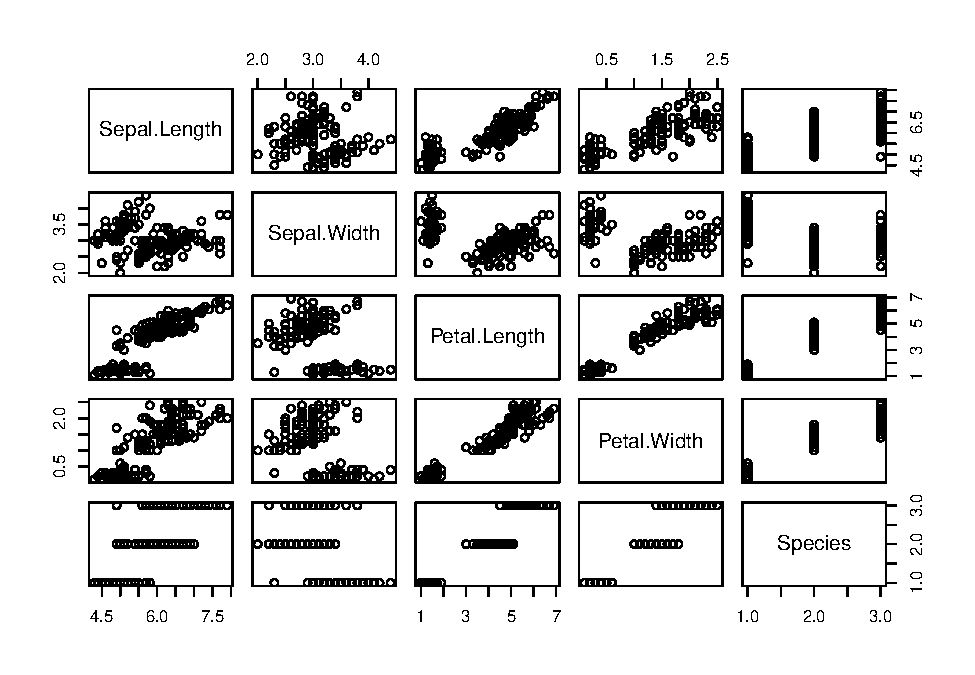
\includegraphics{TCC_files/figure-latex/unnamed-chunk-1-1.pdf}

\newpage

Este texto tem como base: (Brochu, Cora, and De Freitas 2010), (Snoek,
Larochelle, and Adams 2012) e (Ebden 2015)

\hypertarget{introduuxe7uxe3o}{%
\section{Introdução}\label{introduuxe7uxe3o}}

Os algoritmos de Machine Learning raramente não possuem parãmetros, como
por exemplo, a taxa de aprendizado. Muitas vezes esses parâmetros são
considerados nuances.

A optimização bayesiana é um método para encontrar o ponto máximo de
funções, esta técnica utiliza-se de suposições a priori da função em
análise e combina com evidências dos dados para obter a posteriori. ~

No campo da optimização tem-se como objetivo:

\[
\max\limits_{{x \in A \subset \mathbb{R}^d}} f(x)
\]

Normalmente, pressupõe-se que a função objetivo tem uma representação
matemática conhecida, é convexa ou é pelo menos barata para avaliar. No
campo de Machine Learning, uma parte das funções de custo estudadas não
seguem essas suposições. Muitas vezes, a avaliação da função custo é
muito cara(demorada) ou até mesmo impossível, e as propriedas da função
custo são desconhecidas.\\

A optimização bayesiana é útil quando a avaliação da função tem custo
alto, quando não é conhecido as derivadas da função em análise, quando a
função não é convexa ou até mesmo desconhecida.\\

As técnicas de otimização bayesiana são algumas das abordagens mais
eficientes em termos do número de avaliações de funções necessárias. É
conhecida com este nome por ter como base o teorema de Bayes que diz que
a posteriori de um modelo(M) dada evidência dos dados(E) é proporcional
à verossimilhança de E dado M vezes a priori do modelo(M):

\[
P(M|E) \propto P(E|M)P(M)
\]

Na optimização bayesiana, a priori que é definida está ligada ao espaço
que acredita-se que a função de custo possa variar. Mesmo que esta
função seja desconhecida, é razoavel supor que exista conhecimento
prévio sobre alguma de suas propriedades, como a suavidade, isto torna
algumas funções objetivas mais prováveis que outras.\\

Define-se \(x_i\) sendo a i-ésima amostra, e \(f(x_i)\) a observação da
função objetiva em \(x_i\). Serão acumulados as observações
\(D_{i:t}=\left\{ x_{i:t},f(x_{1:t}) \right\}\), a distribuição apriori
será combinada com a verossimilhança \(P(D_{i:t}|f)\), que para
facilitar, pode-se pensar que a verossimilhança é a proprabilidade do
que vimos ocorrer dado que o que achamos sobre a função é a realidade.
Se a nossa crença anterior é que a função objetiva é muito suave e
isenta de erros, os dados com alta variância ou oscilações devem ser
considerados menos prováveis do que os dados que mal se desviam da
média. Agora, podemos combiná-los para obter nossa distribuição
aposteriori:

\[
P(f|D_{1:t}) \propto P(D_{1:t}|f)P(f)
\]

\begin{figure}
\centering
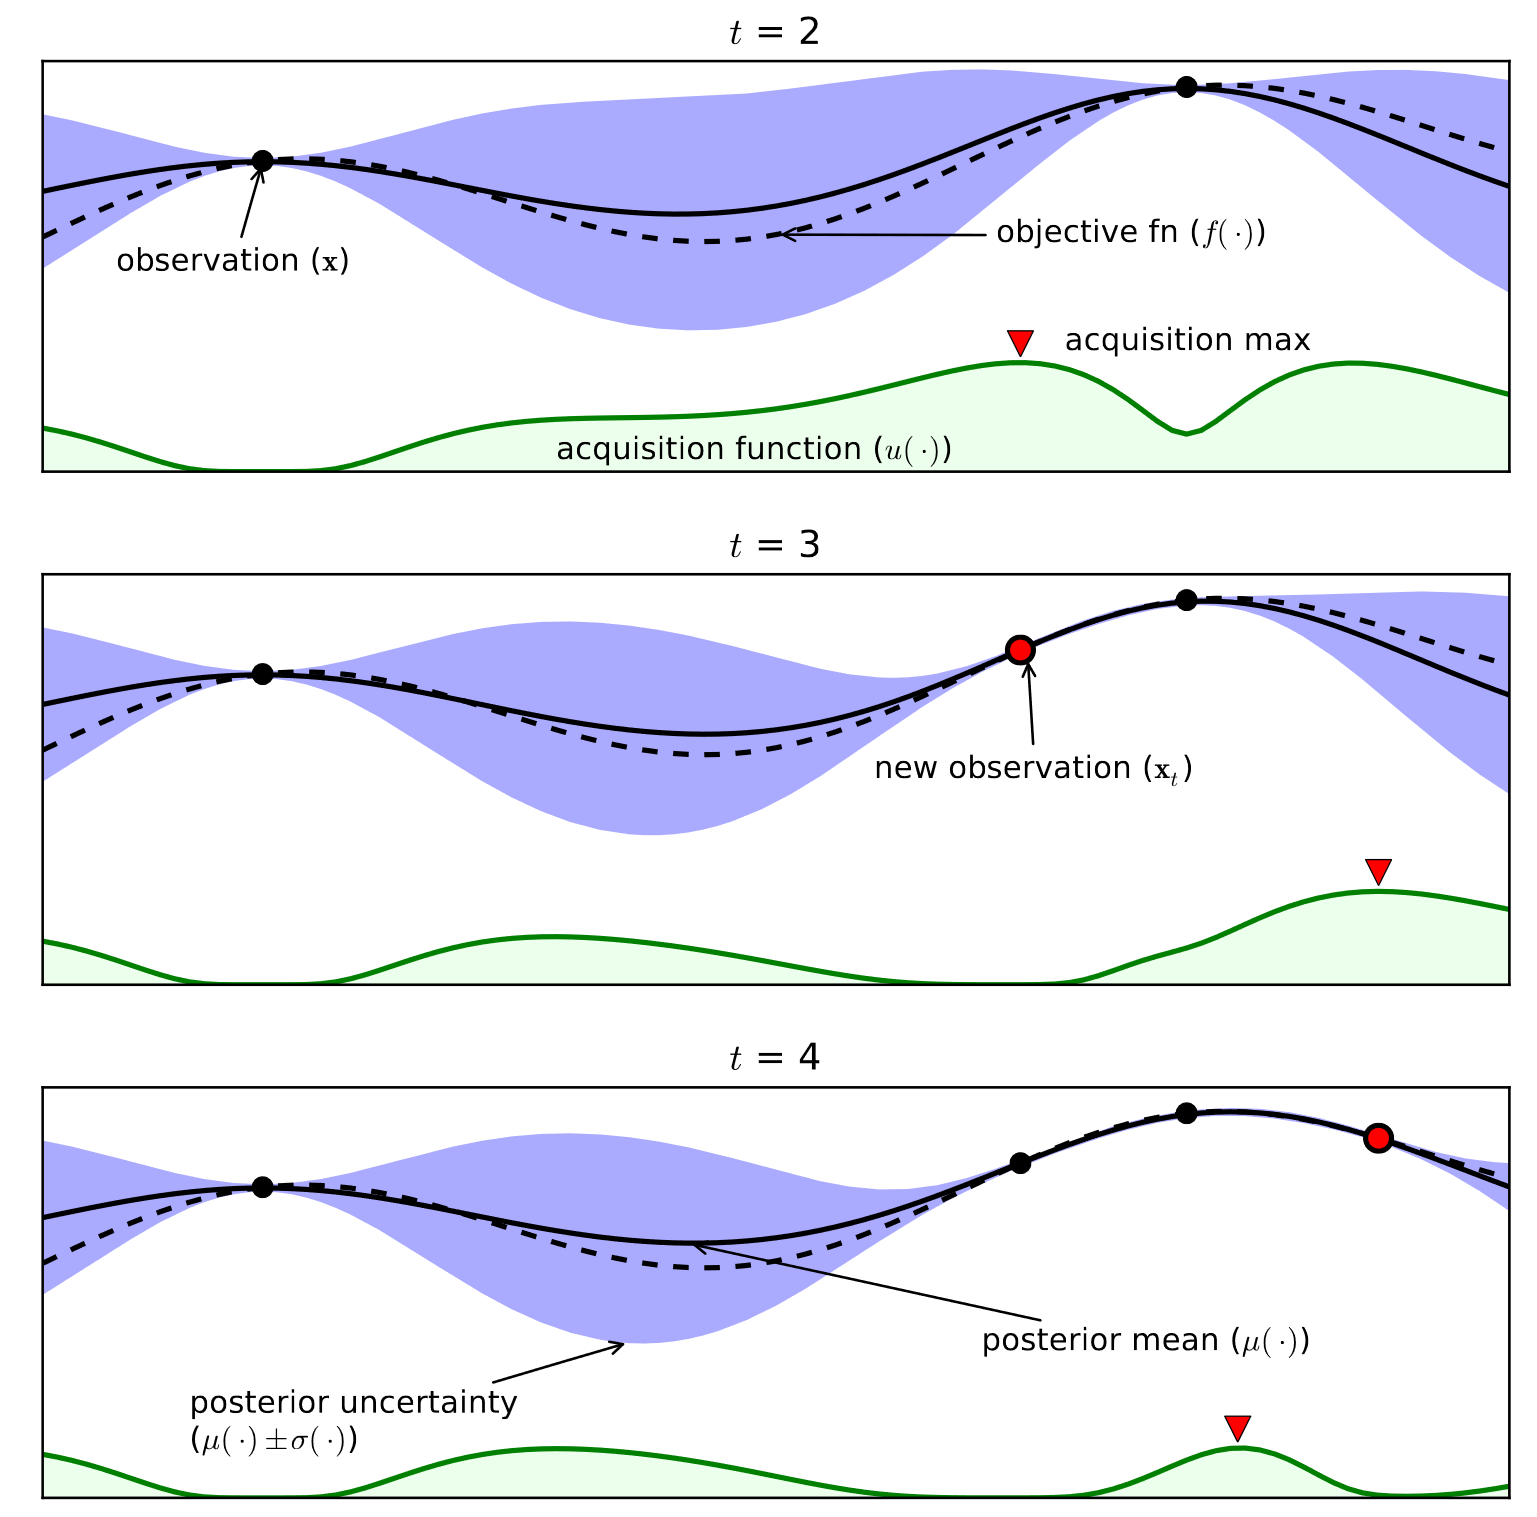
\includegraphics[width=\textwidth,height=0.5\textheight]{images/bo.png}
\caption{Um exemplo do uso da otimização bayesiana em um problema de
design de brinquedo 1D. As figuras mostram uma aproximação do processo
Gaussiano (GP) da função objetivo sobre quatro iterações dos valores
amostrados da função objetivo. A figura também mostra o função de
aquisição nas parcelas sombreadas mais baixas. A aquisição é alta onde o
GP prevê um objetivo elevado (exploração) e onde a incerteza de previsão
é alta (exploração) - áreas com os dois atributos são amostradas
primeiro. Note que a área no extrema esquerda permanece sem amostragem,
como enquanto ele tem alta incerteza, é (corretamente) previsto para
oferecer pouca melhoria sobre a mais alta observação.}
\end{figure}

A posteriori captura a apriori atualizada da função objetivo. Para que
uma amostra eficiente seja obtida é utilizado uma função de aquisição
para determinar o próximo ponto \(x_{t+1} \in A\). A decisão representa
um trade-off automático entre exploração (onde a função objetivo é muito
incerta) e exploração (tentando valores de \(x\) onde a função objetivo
deve ser alta). A optimização bayesiana tem como objetivo minimizar a
quantidade de interações nescessárias para localizar o ponto máximo e
também se comporte bem em funções com múltiplos pontos de máximo.\\
~\\

A figura 1 representa um uma optimização de uma dimensão, onde é
iniciado com dois ponto aleatórios. A cada iteração, a função de
aquisição é maximizada para determinar o pŕoximo ponto para a amostra da
função objetivo. A função de aquisição leva em consideração a média a
posteriori calculada para os pontos e a variância da previsão. E então é
amostrado o \(\operatorname{argmax}\) da função da função de aquisição,
o processo gaussiano é atualizado e o processo é repetido para os
próximos passos.\\
~\\
~\\

\hypertarget{metodologia}{%
\section{Metodologia}\label{metodologia}}

\hypertarget{processos-gaussianos}{%
\section{Processos Gaussianos}\label{processos-gaussianos}}

Os processos gaussianos comunmente são utilizados como para interpolação
de pontos não linear, sendo assim, o objetivo é prever pontos no espaço
não observados, levando em conta que pontos próximos aos observados não
devem mudar bruscamente o valor da variável de interesse. Abaixo será
apresentado um exemplo.\\

\begin{figure}
\centering
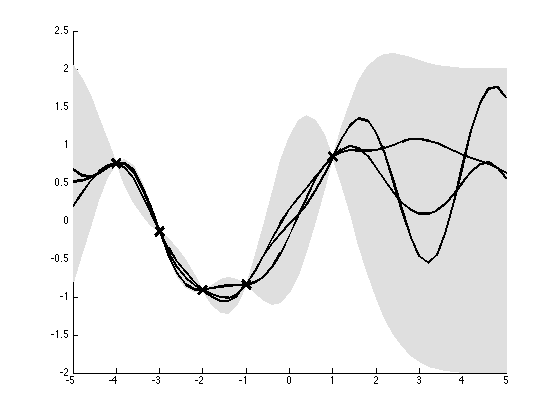
\includegraphics[width=\textwidth,height=0.5\textheight]{images/gp.png}
\caption{\href{https://github.com/probml/pmtk3/blob/30d7a1952f3979b16e92dbfa4cd1ce0e402cf7d8/docs/demoOutput/bookDemos/(15)-Gaussian_processes/gprDemoNoiseFree_02.png}{Retirada
do livro de Kevin Murphy}}
\end{figure}

Podo-se observar, que neste caso, esta sendo considerado que não há
incerteza de medição nos pontos observados represetados pelo \(x\) no
gráfico, as bandas representam um intervalo de confiança de 95\%.\\

`Para o entendimento dos processos gaussianos é nescessário que seja
definido uma noção de similaridade e de variância'

Os processos gaussinaos também podem ser utilizados como distribuição a
priori para uma conjunto de pontos no espaço.\\

Pode-se imaginar como exemplo \(n\) ponto gerados de uma distribuição
n-dimensional normal multivariada, agora imaginando pontos de um domínio
contínuo tem-se um processo gaussiano sendo a generalização
infinito-dimensional de uma variável multi-dimensional gaussiana.\\

A optimização bayesiana utiliza como priori o Processo Gaussiano com o
vetor de médias 0 para facilitar as contas, porém, um fato interessante
do processo gaussiano é que este pode ser totalmente definido pela sua
matriz de covariância.\footnote{Bishop (2012)}\\

A matriz de covariância de um processo gaussiano depende de qual
kernel(K) será utilizado, um dos mais utilizado é o gaussiano, que
possui este nome por ter o mesmo formato da distribução
normal(gaussiana) tendo como única diferença a constnate de
normalização, definido a seguir.\\

\[
X \sim GP(0,\Sigma)
\]

\[
\Sigma(x_1,x_2) = K(x_1,x_2) + I\sigma^2_y
\]

\[
K(x_1,x_2) = \sigma^2 e^{-\frac{1}{2l^2}(x_1-x_2)^2}
\]

\hypertarget{funuxe7uxe3o-de-aquisiuxe7uxe3o}{%
\section{Função de aquisição}\label{funuxe7uxe3o-de-aquisiuxe7uxe3o}}

Será assumido que a função \(f(x)\) é uma observação de um processo
gaussiano e que as observações, \((x_n,y_n)_{n=1}^N\), onde
\(y_n \mbox{~} N(f(x_n),\nu)\) e \(\nu\) é a variância dos ruídos
introduzidos na função de observação. Utilizando a regra de bayes para
combinar a proiri com os dados para gerar a posteriori que determina
qual ponto de \(\chi\)

\newpage

\hypertarget{referuxeancias}{%
\section*{Referências}\label{referuxeancias}}
\addcontentsline{toc}{section}{Referências}

\hypertarget{refs}{}
\leavevmode\hypertarget{ref-bishop2012pattern}{}%
Bishop, Christopher M. 2012. ``Pattern Recognition and Machine Learning,
2006.'' \emph{Korean Society of Civil Engineers} 60 (1): 78--78.

\leavevmode\hypertarget{ref-brochu2010tutorial}{}%
Brochu, Eric, Vlad M Cora, and Nando De Freitas. 2010. ``A Tutorial on
Bayesian Optimization of Expensive Cost Functions, with Application to
Active User Modeling and Hierarchical Reinforcement Learning.''
\emph{arXiv Preprint arXiv:1012.2599}.

\leavevmode\hypertarget{ref-ebden2015gaussian}{}%
Ebden, Mark. 2015. ``Gaussian Processes: A Quick Introduction.''
\emph{arXiv Preprint arXiv:1505.02965}.

\leavevmode\hypertarget{ref-snoek2012practical}{}%
Snoek, Jasper, Hugo Larochelle, and Ryan P Adams. 2012. ``Practical
Bayesian Optimization of Machine Learning Algorithms.'' In
\emph{Advances in Neural Information Processing Systems}, 2951--9.

% ----------------------------------------------------------
% ELEMENTOS PÓS-TEXTUAIS
% ----------------------------------------------------------
\postextual

% ----------------------------------------------------------
% Referências bibliográficas
% ----------------------------------------------------------
\bibliography{bibliography.bibtex}

\phantompart

\printindex

\end{document}
